\documentclass[10pt]{standalone}
\usepackage{amsmath}
\usepackage{pgf,tikz}
\usepackage{mathrsfs}
\usetikzlibrary{arrows}
\pagestyle{empty}
\begin{document}

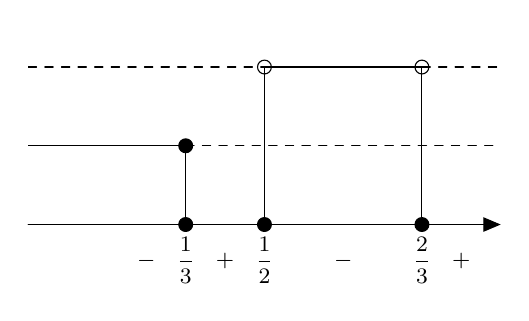
\begin{tikzpicture}[line cap=round,line join=round,>=triangle 45,x=1.0cm,y=1.0cm]
\draw[->,color=black] (-3.,0.) -- (3.,0.);
%\foreach \x in {-3.,-2.,-1.,1.,2.}
%\draw[shift={(\x,0)},color=black] (0pt,2pt) -- (0pt,-2pt) node[below] {\footnotesize $\x$};
%\draw[->,color=black] (0.,-0.8) -- (0.,2.5);
%\foreach \y in {,1.,2.}
%\draw[shift={(0,\y)},color=black] (2pt,0pt) -- (-2pt,0pt) node[left] {\footnotesize $\y$};
\draw[color=black] (0pt,-13pt) node {\footnotesize $\dfrac{1}{2}$};
\draw[color=black] (-1,-13pt) node {\footnotesize $\dfrac{1}{3}$};
\draw[color=black] (2,-13pt) node {\footnotesize $\dfrac{2}{3}$};
\draw[color=black] (-1.5,-13pt) node {\footnotesize $-$};
\draw[color=black] (-0.5,-13pt) node {\footnotesize $+$};
\draw[color=black] (1,-13pt) node {\footnotesize $-$};
\draw[color=black] (2.5,-13pt) node {\footnotesize $+$};
\clip(-3.,-0.8) rectangle (3.,2.5);
\draw [dash pattern=on 3pt off 3pt] (-1.,1.)-- (3.,1.);
\draw (-1.,1.)-- (-1.,0.);
\draw (-3.,1.)-- (-1.,1.);
\draw [dash pattern=on 3pt off 3pt] (-3.,2.)-- (0.,2.);
\draw (0.,2.)-- (2.,2.);
\draw [dash pattern=on 3pt off 3pt] (2.,2.)-- (3.,2.);
\draw (0.,2.)-- (0.,0.);
\draw (2.,2.)-- (2.,0.);
\begin{scriptsize}
\draw [fill=black] (-1.,1.) circle (2.5pt);
\draw  (0.,2.) circle (2.5pt);
\draw  (2.,2.) circle (2.5pt);
\draw [fill=black] (-1.,0.) circle (2.5pt);
\draw [fill=black] (0.,0.) circle (2.5pt);
%\draw[color=black] (0.14,0.37) node {$I$};
%\draw[color=black] (-0.26,1.17) node {$m$};
\draw [fill=black] (2.,0.) circle (2.5pt);
%\draw[color=black] (2.14,0.37) node {$J$};
\end{scriptsize}
\end{tikzpicture}
\end{document}